\chapter{Deployment}\label{ch:deployment}

The deployment phase of this project involved the successful installation and integration of the parking management system across ten different communities in Valencia. This chapter details the deployment process, challenges encountered, and solutions implemented to ensure system reliability across diverse environments. 

\section{Deployment Process}

The deployment of new communities follows a standardized four-phase approach to ensure consistency and reliability. The initial phase involves physical hardware installation, including the NVIDIA Jetson Nano, cameras, networking equipment, and relay systems. Careful consideration is given to equipment placement, particularly for cameras, to optimize license plate recognition while protecting hardware from environmental factors. 

The second phase focuses on establishing network connectivity and integrating the community into the broader system architecture. This includes configuring the 4G router, setting up ZeroTier connections, and verifying communication with the central server. Each community receives a unique identifier within the network to maintain proper isolation and security. 

The third phase encompasses data population and system configuration through the web interface. This involves adding authorized users, registering license plates, and configuring community-specific parameters such as parking space limits and access rules. Administrator training is conducted during this phase to ensure proper system management. 

The final phase involves system validation and monitoring. During this period, the system operates under close supervision to verify all components function correctly and to address any community-specific requirements or issues that arise.

\section{Environmental Challenges}

Deployment across multiple communities revealed significant environmental challenges that impacted system reliability. The Dana weather event in Valencia in September 2024 \autocite{CNNSpainFlooding2024} severely affected three communities, where flooding damaged terminal equipment and disrupted system operations, see \cref{fig:dana}. This experience led to the implementation of enhanced waterproofing measures and the elevation of critical hardware components above potential flood levels. 

\begin{figure}
        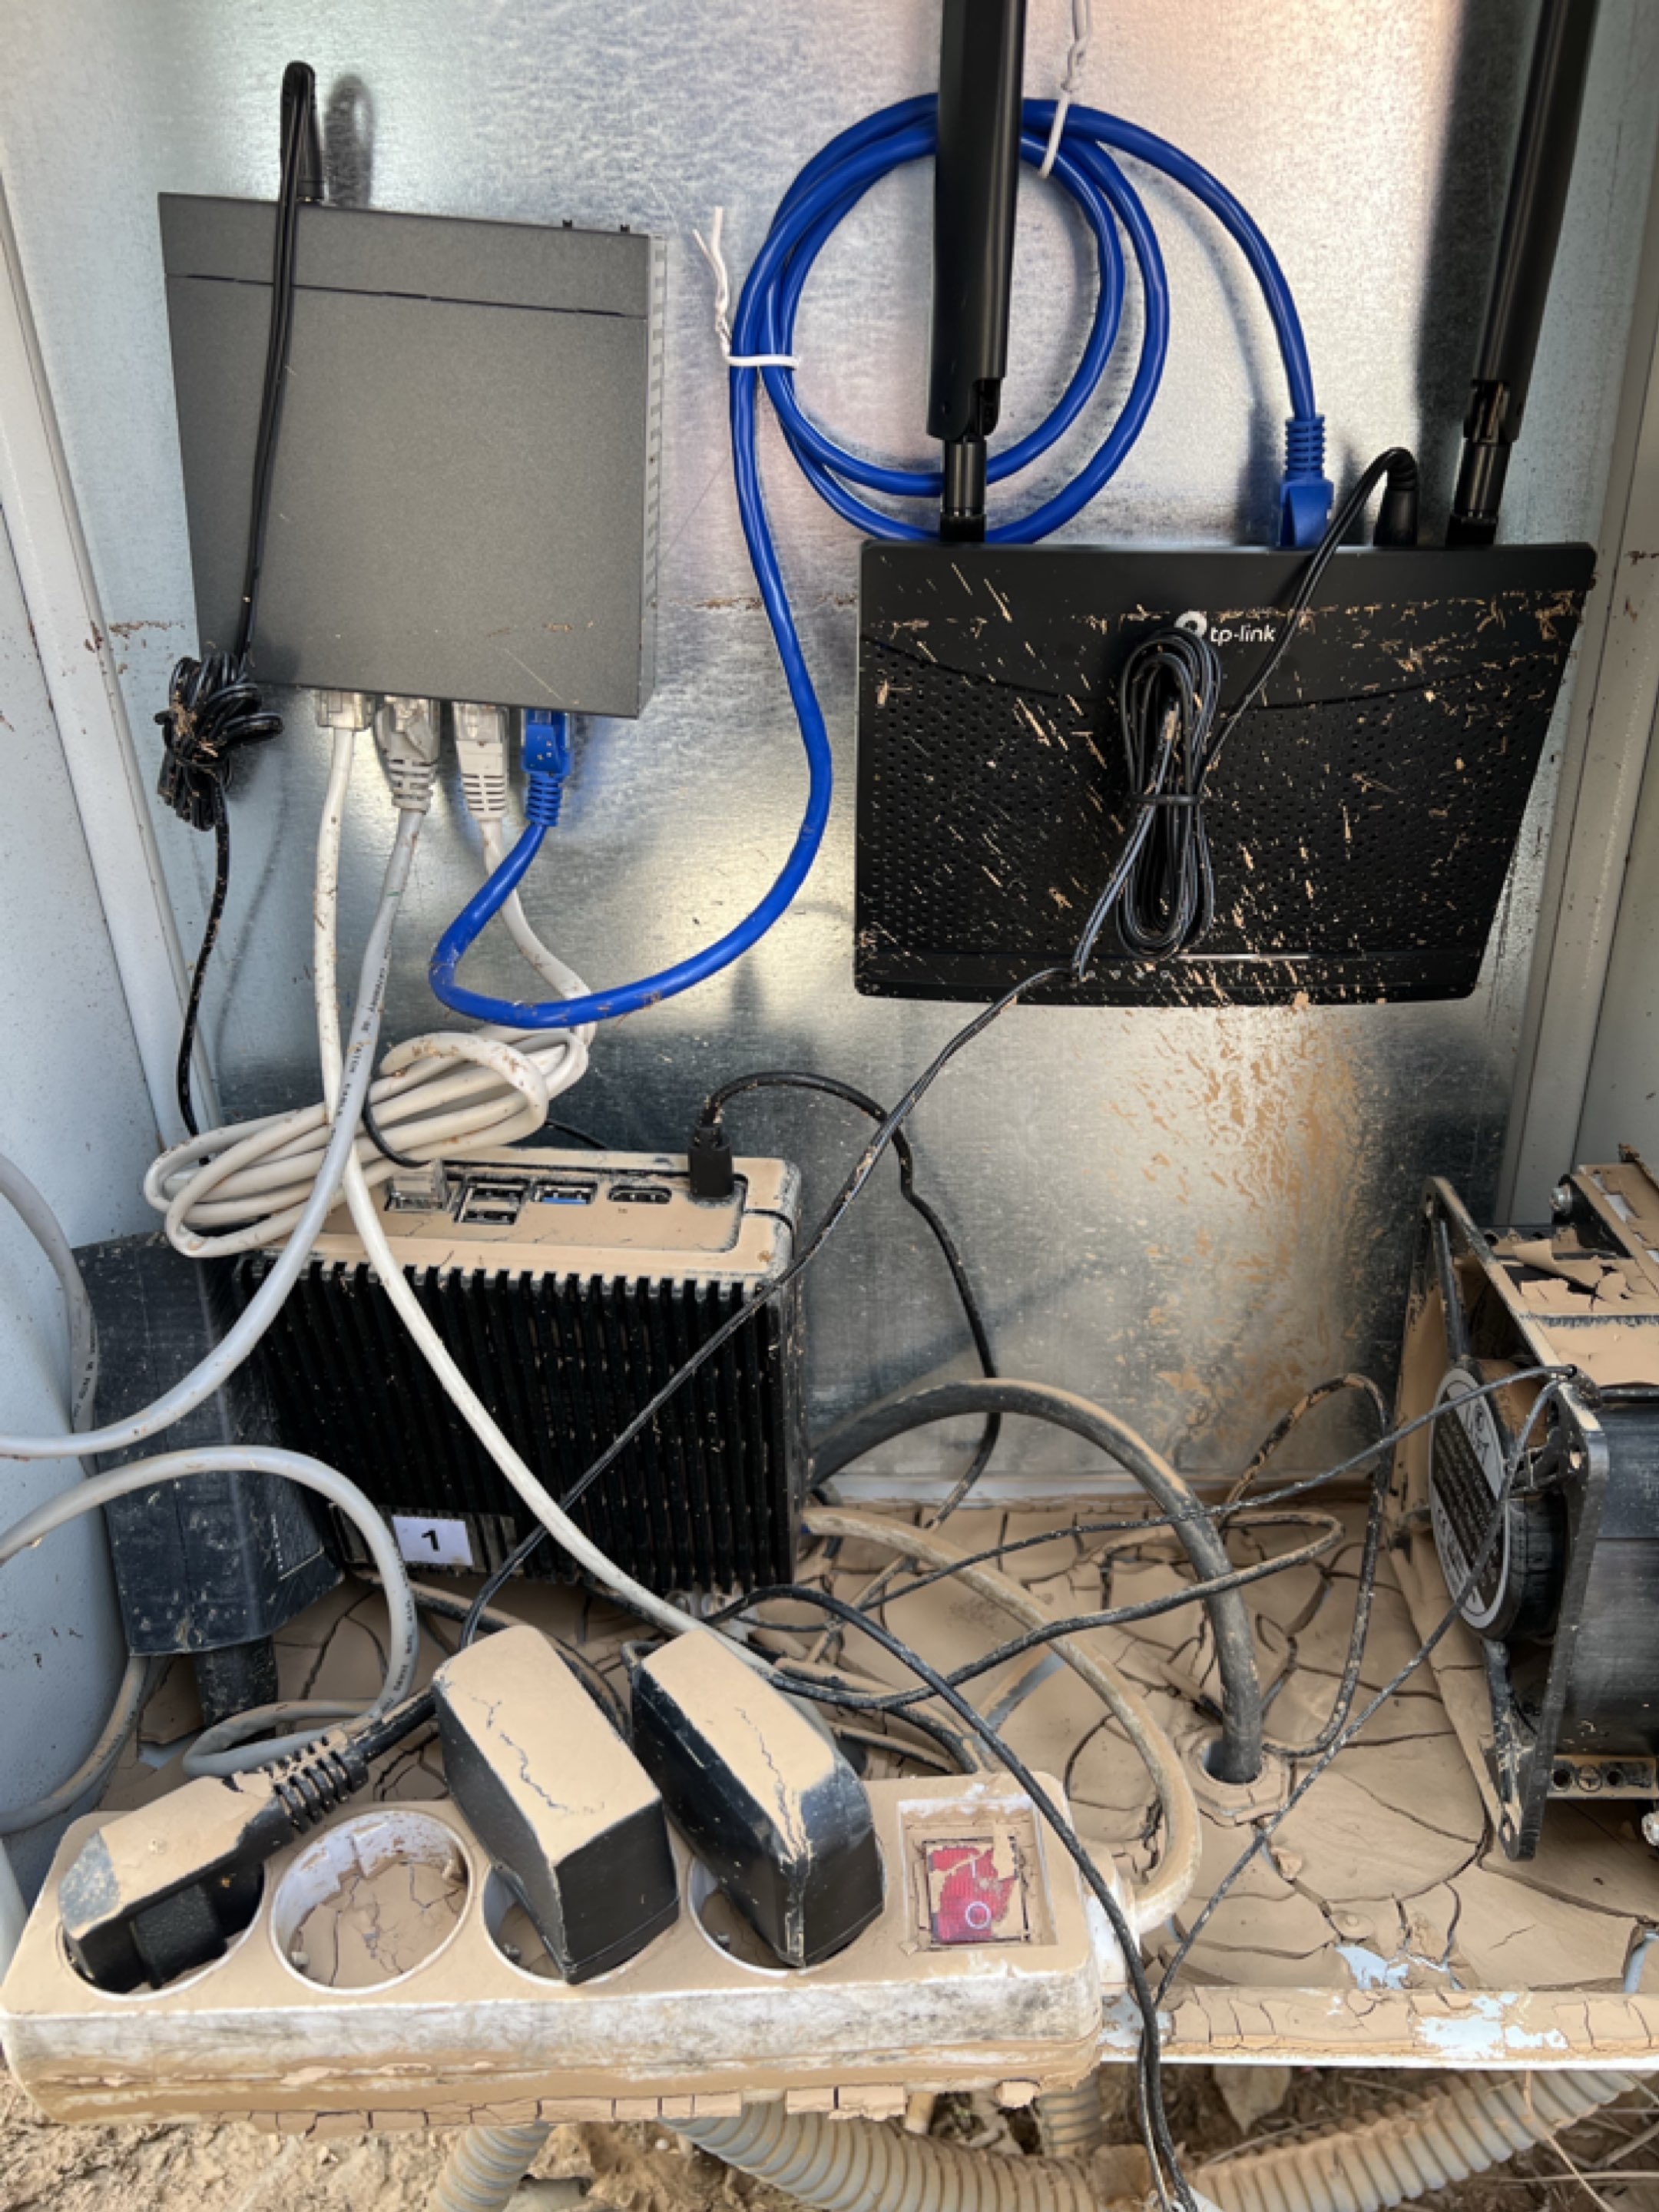
\includegraphics{dana.jpg}
    \caption{Dana weather event in one of the communities in Valencia, September 2024}\label{fig:dana}
\end{figure}

Camera performance was notably affected by varying weather conditions. Direct sunlight caused glare issues that impacted license plate recognition accuracy, while heavy rain sometimes triggered false readings as water made the lense blurry \cref{fig:wet_camera}. These challenges were addressed through the installation of protective shields and the refinement of the recognition algorithms to account for adverse weather conditions. 

\begin{figure}
        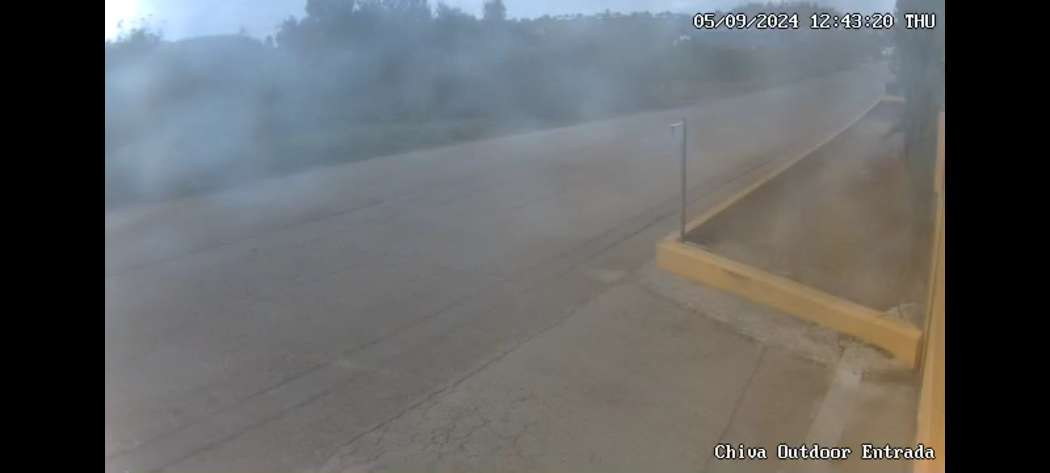
\includegraphics{empanado.jpg}
    \caption{Water leakage inside a camera making the image blurry}\label{fig:wet_camera}
\end{figure}

\section{Community-Specific Adaptations}

Different communities presented unique infrastructure requirements that necessitated system adaptations. Several communities required dual garage door configurations to manage separate entry and exit points. This led to the development of enhanced traffic flow management algorithms and modified hardware setups to coordinate multiple access points effectively. 

The installation process revealed varying electrical infrastructure across communities, requiring custom solutions for power delivery and surge protection. In older buildings, existing wiring needed to be carefully evaluated and sometimes upgraded to support the system's power requirements while maintaining safety standards.


